% vim: set textwidth=78 autoindent:

\section{Lavorare con i dati OGC}

% when the revision of a section has been finalized, 
% comment out the following line:
%\updatedisclaimer

QGIS supporta sorgenti di dati WMS e WFS. Il supporto WMS è nativo, quello per
WFS è fornito tramite plugin.

\subsection{Cosa sono i dati OGC}\index{OGC!introduzione}

L'Open Geospatial Consortium (OGC), è un’organizzazione internazionale che raggruppa più
di 300 organizzazioni commerciali, governative, nonprofit e di ricerca.
I suoi membri sviluppano e implementano standard per contenuti e servizi geospaziali,
analisi GIS e scambio dati.

Dal Consorzio è stato quindi elaborato un numero crescente di specifiche per i modelli di
dati per garantire bisogni specifici riguardanti l'interoperabilità
nell'ambito della tecnologia geospaziale, inclusi i GIS. Ulteriori
informazioni all'indirizzo \url{http://www.opengeospatial.org/}.

Importanti specifiche OGC sono:

\begin{itemize}
\item \textbf{WMS} - Web Map Service
\item \textbf{WFS} - Web Feature Service
\item \textbf{WCS} - Web Coverage Service
\item \textbf{CAT} - Web Catalog Service
\item \textbf{SFS} - Simple Features for SQL
\item \textbf{GML} - Geography Markup Language
\end{itemize}

Ad oggi i servizi OGC-sono sempre più di uso comune per scambiare dati geografici fra
differenti implementazioni GIS. QGIS ora può gestire tre delle specifiche esposte sopra
tra cui SFS (tramite il supporto a PostgreSQL/PostGIS, vedi Sezione
\ref{label_postgis}); e WFS e WMS come client.


\subsection{Client WMS}\label{sec:ogc-wms}\index{WMS!client}\index{OGC!WMS!client}\index{raster!WMS}

\subsubsection{Panoramica sul servizio WMS}\label{sec:ogc-wms-about}\index{WMS!client!considerazioni}

QGIS può agire come client WMS, nel rispetto delle specifiche 1.1, 1.1.1 e 1.3.
È stato particolarmente testato nei confronti di server accessibili pubblicamente
quali DEMIS e JPL OnEarth.

I server WMS rispondono alle richieste da parte dei client (ad es. QGIS) di una mappa raster
di una determinata estensione, con un determinato insieme di layer, simboli e trasparenze.
Il server WMS quindi consulta le sue risorse (locali o remote), genera il raster e lo invia
al client in formato raster, per QGIS tipicamente come immagini JPEG o PNG.

WMS è un servizio REST (Representational State Transfer) piuttosto che un servizio web completo.
Come tale, si può prendere la URL (indirizzo del server con specifiche) generata da QGIS e usarla
in un browser web per ottenere la stessa immagine che QGIS usa internamente. Questo può essere
utile per identificare le cause di eventuali problemi, dato che esistono vari tipi di server
WMS e ciascuno ha la sua propria interpretazione degli standard WMS.

I layer WMS possono essere aggiunti molto semplicemente, una volta
disponibile l'indirizzo (URL) per accedere al server WMS, una connessione adatta
e posto che il server usi l’HTTP come meccanismo di trasferimento dati.

\subsubsection{Scegliere un server WMS}\label{sec:ogc-wms-servers}\index{WMS!server remoto!selezionare}

La prima volta in cui si vuole utilizzare un servizio WMS, non sono presenti
server predefiniti. Si può avviare lo strumento cliccando sul pulsante
\toolbtntwo{mActionAddWmsLayer}{Aggiungi layer WMS} nella barra strumenti, 
oppure dalla voce di menu
\mainmenuopt{Layer}>\dropmenuopttwo{mActionAddWmsLayer}{Aggiungi layer WMS...}.
Si aprirà la finestra di dialogo \dialog{Aggiungi layer dal server}. È
possibile aggiungere alcuni server cliccando sul pulsante
\button{Aggiungi server predefiniti}. Verranno quindi aggiunti almeno tre
server WMS, incluso il server della NASA (JPL). Per definire un nuovo server WMS
nella sezione \tab{Connessioni server}, cliccare su \button{Nuovo} ed inserire
i parametri di connessione al server WMS desiderato, seguendo le indicazioni della
tabella \ref{tab:wms_connection_parms}:

\begin{table}[ht]\index{WMS!client!parametri connessione}
\centering
\caption{Parametri connessione WMS}\label{tab:wms_connection_parms}\medskip
 \begin{tabular}{|l|p{5in}|}
\hline Nome & nome per la connessione che consenta di individuarlo nella
lista dei server WMS nel menu a tendina. \\
\hline URL \index{WMS!URL} &  indirizzo URL del server che fornisce i dati.
Deve essere un indirizzo raggiungibile, nello stesso formato che verrebbe
usato per aprire una connessione telnet o pingare un host. \\
\hline
\end{tabular}
\end{table}

È possibile, se necessario, impostare nelle opzioni i parametri del proxy per ricevere i servizi WMS da internet.
Selezionare la voce di menu \mainmenuopt{Impostazioni} >
\dropmenuopttwo{mActionOptions}{Opzioni} e cliccare sulla scheda
\tab{Proxy}, nella quale è possibile inserire le impostazioni abilitando la
casella di controllo \checkbox{Utilizza un proxy per l'accesso web}.

Una volta creata la connessione al server WMS, essa sarà memorizzata e
disponibile per le successive sessioni di QGIS.

\begin{Tip}[ht]\caption{\textsc{A proposito di indirizzi dei server WMS}}
\qgistip{Quando si inserisce l'indirizzo URL del server assicurarsi di
usare l'indirizzo di base. Ad esempio non bisogna inserire frammenti tipo
\usertext{request=GetCapabilities} o \usertext{version=1.0.0} nell'indirizzo.\index{WMS!server remoto!URL}
}
\end{Tip}

La tabella \ref{tab:wms_example_urls} mostra alcuni esempi di indirizzi di
server WMS con i quali iniziare.
Questi links sono stati controllati l'ultima volta nel Dicembre 2006, ma
potrebbero essere stati modificati nel frattempo:

%FIXME:  WMS URLs should be checked again and maybe extended in QGIS 

\begin{table}[ht]\index{WMS!server remoto!esempi URL}
\centering
\caption{Esempi di indirizzi di server WMS pubblici}\label{tab:wms_example_urls}\medskip
 \begin{tabular}{|l|l|}
\hline \textbf{Name}        & \textbf{URL} \\
\hline Atlas of Canada      & http://atlas.gc.ca/cgi-bin/atlaswms\_en? \\
\hline DEMIS                & http://www2.demis.nl/wms/wms.asp?wms=WorldMap\& \\
\hline Geoscience Australia & http://www.ga.gov.au/bin/getmap.pl?dataset=national \\
\hline NASA JPL OnEarth     & http://wms.jpl.nasa.gov/wms.cgi? \\
\hline QGIS Users           & http://qgis.org/cgi-bin/mapserv?map=/var/www/maps/main.map\& \\
\hline
\end{tabular}
\end{table}

Un elenco esaustivo di server WMS è reperibile all'indirizzo \url{http://wms-sites.com}.

\subsubsection{Caricare layer WMS}\label{sec:ogc-wms-layers}\index{WMS!client!layer}

Una volta compilati correttamente i campi, si può premere sul pulsante
\button{Connetti} per ottenere le capacità del server. Tra queste sono inclusi
i formati immagine, i layer disponibili e i sistemi di proiezione forniti dal
server. Considerato che si tratta di operazioni in rete, la velocità nella
risposta dipenderà dalla qualità della connessione verso il server WMS. Mentre
si scaricano i dati dal server, l'avanzamento dell'operazione viene
visualizzato nella porzione inferiore sinistra della finestra. 

Lo schermo dovrebbe rassomigliare alla Figura \ref{fig:connection_wms}, che
mostra la risposta fornita dal server WMS NASA JPL OnEarth.

\begin{figure}[ht]
  \begin{center}
  	\caption{Finestra per l'aggiunta di un server WMS, nella quale vengono
	mostrati i layer disponibili \nixcaption}\label{fig:connection_wms}
	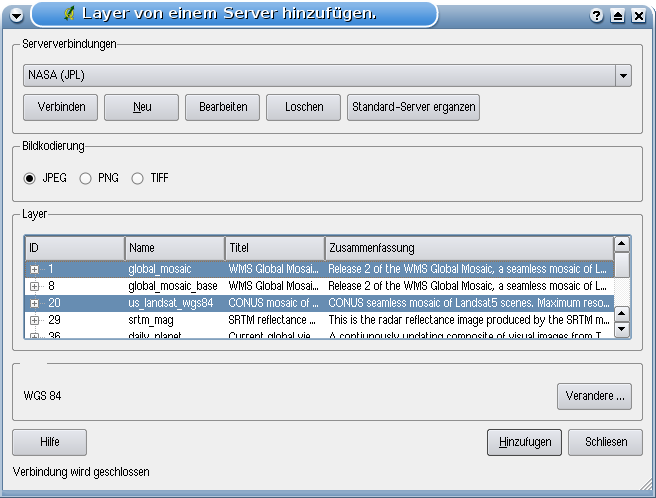
\includegraphics[clip=true,width=0.6\textwidth]{connection_wms}
  \end{center}
\end{figure}

\minisec{Codifica immagine}

La sezione \tab{Codifica immagine} elenca i formati supportati sia dal client
che dal  server. La scelta dipenderà dalla risoluzione che necessita allo scopo
prefisso.

\begin{Tip}[ht]\caption{\textsc{Codifica immagine}}
\qgistip{Solitamente un server WMS offrirà la scelta tra le codifiche JPEG e
PNG. Mentre la compressione JPEG comporta una perdita di qualità, quella PNG
riproduce fedelmente il dato di origine. Usare JPEG se non interessa avere una
certa perdita di qualità dell'immagine, riducendo d'altro canto il tempo per
il download dei dati di 5 volte rispetto al formato PNG. Usare invece PNG se
si vuole una rappresentazione precisa del dato originale e non ci si preoccupa
del tempo necessario per il trasferimento dei dati.
\index{WMS!codifica immagine}
}
\end{Tip}

\minisec{Layers}

La sezione \tab{Layer} elenca i layer disponibili dal server WMS
selezionato. Si vedrà che alcuni layer sono espandibili, il che comporta che
possono venir mostrati in diversi stili di immagine.

Possono essere selezionati diversi layer alla volta, ma un solo stile di
immagine per ognuno di essi. Quando si effettua una selezione multipla, i
layer vengono richiesti al server e trasmessi a QGIS in un solo blocco.

\begin{Tip}[ht]\caption{\textsc{Ordine dei layer WMS}}
\qgistip{In questa versione di QGIS, i layer WMS caricati sono sovrapposti in
base all'ordine in cui sono elencati nella sezione Layer, dall'alto verso il
basso. Se si desidera sovrapporre i layer nel senso opposto occorre
selezionare una seconda volta \toolbtntwo{mActionAddWmsLayer}{Aggiungi layer
WMS}, scegliere nuovamente lo stesso server e selezionare il secondo gruppo di
layer che si desidera sovrapporre al primo.
\index{WMS!server remoto!ordinamento layer}
}
\end{Tip}

\minisec{Trasparenza}\label{ogc-wms-transparency}

In questa versione di QGIS la trasparenza è impostata per essere sempre
attiva, se disponibile.

\begin{Tip}[ht]\caption{\textsc{Trasparenza dei Layer WMS}}
\qgistip{La possibilità di rendere trasparenti i layer WMS dipenda dalla codifica tramite la quale sono stati caricati: PNG e GIF gestiscono la trasparenza mentre il JPEG no.
\index{WMS!trasparenza layer}
}
\end{Tip}

\minisec{Sistema di proiezione delle coordinate (Coordinate Reference System)}
\index{WMS!CRS}\index{WMS!sistema di proiezione delle coordinate}
\index{OGC!CRS}\index{OGC!sistema di proiezione delle coordinate}
\index{proiezioni!WMS}
\index{proiezioni!CRS}\index{proiezioni!sistema di proiezione delle coordinate}
\index{CRS}\index{sistema di proiezione delle coordinate}
\index{SRS}\index{proiezioni!SRS}

Un sistema di proiezione delle coordinate (Coordinate Reference System, CRS) è
il termine OGC per una proiezione in QGIS.

Ogni layer WMS può essere restituito in molteplici CRS, in funzione delle
capacità del server. Si noti che il numero di sistemi di riferimento tra cui
scegliere viene indicato nella dicitura \textsl{Coordinate Sistema di
Riferimento (x disponibili)} quando si seleziona/deseleziona un livello nella
sezione \tab{Layer}.

Per scegliere uno dei CRS disponibili, cliccare su \button{Cambia...} per fare
apparire una finestra simile a quella della Figura \ref{fig:projections} alla
Sezione \ref{label_projstart}.
La differenza principale rispetto alla versione WMS mostrata nello schermo è
che saranno mostrati solo i CRS supportati dal server al quale ci si sta
effettivamente connettendo.


\begin{Tip}[ht]\caption{\textsc{Le proiezioni WMS}}
\qgistip{Per ottenere i migliori risultati, aggiungere per primo al progetto
il layer WMS, in modo che il sistema di riferimento dell'intero progetto sia
lo stesso attribuito al layer WMS.
Si potrà quindi usare la proiezione al volo (si veda la Sezione \ref{sec:projection-specifying})
per adattare qualunque altro layer vettoriale successivamente aggiunto.
In questa versione di QGIS, aggiungere layer WMS successivamente ad altri
con un CRS diverso rispetto a quello del progetto, può causare errori.
}
\end{Tip}


\subsubsection{Uso dello strumento di identificazione}\label{sec:ogc-wms-identify}
\index{WMS!identificazione}
\index{identificazione!WMS}
\index{WMS!GetFeatureInfo}

Una volta aggiunto un server WMS, e se uno dei layer disponibili è
interrogabile, è possibile usare lo strumento
\toolbtntwo{mActionIdentify}{Informazioni geometrie} per selezionare un pixel
sulla mappa, determinando una interrogazione verso il server WMS per ogni
selezione.

I risultati dell'interrogazione vengono restituiti come testo semplice la cui
formattazione dipenderà dalle impostazioni del server WMS.

% FIXME: GetFeatureInfo-Requests are done here?

\subsubsection{Visualizzazione delle proprietà del server}\label{sec:ogc-wms-properties}\index{WMS!proprietà}
\index{raster!proprietà}

Una volta aggiunto un server WMS, è possibile visualizzarne le le proprietà
cliccando con il tasto destro sul suo nome nella legenda e selezionando
\button{Proprietà}.


\minisec{Scheda Metadata}\label{sec:ogc-wms-properties-metadata}
\index{raster!metadata}
\index{WMS!metadata}
\index{WMS!capacità/capabilities}

La scheda \tab{Metadata} mostra parecchie informazioni sul server WMS,
generalmente raccolte dall'affermazione "Capabilities" ritornata dal server all'apposita richiesta.

Molte definizioni possono essere dedotte leggendo gli standard WMS \cite{OGCWMS010101web}, \cite{OGCWMS010300web}, alcune definizioni utili sono le seguenti:

\begin{itemize}
\item \textbf{Proprietà server}

\begin{itemize}
\item \textbf{Versione WMS}      - La versione WMS supportata dal server.

\item \textbf{Formati immagine}  - Elenco dei tipi MIME che il server può
                                   fornire  per disegnare la mappa. QGIS
				   supporta qualunque formato sia supportato
				   dalle librerie Qt contro le quali è
				   compilato, che sono solitamente almeno \texttt{image/png}
				   e \texttt{image/jpeg}.

\item \textbf{Interroga formati} - L'elenco dei tipi MIME con i quali il server
                                   può fornire risposta quando si usa lo strumento
				   "Identifica geometrie". Attualmente QGIS supporta
				   il tipo \texttt{text-plain}.

\end{itemize}

\item \textbf{Proprietà layer}

\begin{itemize}
\item \textbf{Selezionato}         - Indica se il layer era selezionato quando
                                     il server è stato aggiunto al progetto.

\item \textbf{Visibilità}          - Indica se il layer sia stato impostato
                                     come visibile in legenda.  (funzione non ancora utilizzata
				     in questa versione di QGIS.)

\item \textbf{Può interrogare}     - Indica se il layer fornisca o meno
                                     informazioni se si usa lo strumento "Identifica geometrie".

\item \textbf{Può essere trasparente} - Indica se il layer può essere o meno
                                        reso trasparente a video. Questa
					versione di QGIS farà sempre uso della
					trasparenza se questa voce visualizza
					\textsl{Sì} e se il formato immagine
					la supporta.
% BM: doesn't seem to work?
%                                    (see Section
%                                    \ref{ogc-wms-transparency}
%                                    ).

\item \textbf{Può ingrandire}      - Indica se questo layer possa o meno
                                     essere ingrandito dal server.
				     Questa versione di QGIS suppone che tutti i
                                     layer WMS abbiano questa opzione settata su \textsl{Sì}.
                                     Layers carenti in questa impostazione
				     possono essere resi a video in modo
				     anomalo.

\item \textbf{Conteggio a cascata}    - I server WMS possono fungere da proxy
                                        per altri server WMS dai quali ottengono
					i dati raster per un certo layer. La
                                        voce mostra quindi quante richieste per questo
					layer vengono inoltrate ai nodi
                                        per ottenere un risultato.

\item \textbf{Larghezza fissa}, \textbf{Altezza fissa}
                                - Indica se lo layer abbia o meno una
				dimensione del pixel fissata alla sorgente.
                                  Questa versione di QGIS assume che tutti i
				  layer WMS abbiano vuota questa voce. Layers
				  con impostazioni diverse possono essere resi
				  a video in modo anomalo.

\item \textbf{Perimentro WGS 84} - Estensione del layer in coordinate WGS84. Alcuni server
                                   WMS non settano questo parametro correttamente (ad
				   es. usano coordinate UTM invece di WGS84).
				   In questo caso sembrerà che la vista
				   iniziale del layer
                                   sia ad uno zoom molto ridotto. Bisognerebbe
				   informare di questi errori il webmaster del
				   server WMS, il quale li dovrebbe
				   identificare come elementi
				   WMS XML \texttt{LatLonBoundingBox},
				   \texttt{EX\_GeographicBoundingBox} o CRS:84 \texttt{BoundingBox}.

\item \textbf{Disponibile in CRS} - Sistemi di proiezione nel quale il layer
                                    può essere rappresentato dal server WMS,
				    elencati nel formato nativo WMS.

\item \textbf{Disponibile in stile} - Stili visuali applicabili al layer dal server WMS.

\end{itemize}

\end{itemize}


\subsubsection{Limitazioni del client WMS}\label{sec:ogc-wms-limits}\index{WMS!client!limitazioni}

Non tutte le possibili funzionalità WMS sono state incluse in questa versione di QGIS. Le eccezioni
più rilevanti sono:

\minisec{Modificare le impostazioni del layer WMS}
\index{WMS!impostazioni layer!modifica}

Una volta completata la procedura mostrata dalla finestra
\toolbtntwo{mActionAddWmsLayer}{Aggiungi layer WMS}, non è più possibile
modificarne i parametri.

Una possibile soluzione è quella di eliminare il layer completamente e
ricaricarlo reimpostando i parametri.

\minisec{Server WMS che richiedono un'autenticazione}
\index{WMS!server remoto!autenticazione}

Sono accessibili solo server pubblici. Non è infatti possibile impostare user
name e password per l'autentificazione al server WMS.

\begin{Tip}[ht]\caption{\textsc{Accesso a layer OGC con password}}
\qgistip{Se fosse necessario accedere a layer protetti con password, è
possibile usare InteProxy come proxy trasparente, che supporta molti metodi
di autenticazione. Ulteriori informazioni sono fornite dal manuale di
InteProxy al sito web \url{http://inteproxy.wald.intevation.org}.
\index{WMS!layer protetti!}\index{OGC!autenticazione}
}
\end{Tip}


\subsection{Client WFS}

In QGIS, un layer WFS si comporta come un qualsiasi altro layer vettoriale.
È possibile identificare e selezionare elementi e visualizzare la tabella
attributi. L'unica eccezione è che al momento non è supportata la modifica del
layer. Per avviare il plugin the WFS bisogna andare alla voce di menu
\mainmenuopt{Plugins} > \dropmenuopttwo{mActionShowPluginManager}{Gestione
Plugins...}, attivare la casella di controllo \checkbox{plugin WFS} e cliccare su \button{OK}. 

Apparirà nella barra una nuova icona per lo strumento
\toolbtntwo{mIconAddWfsLayer}{Aggiungi layer WFS} vicino all'icona WMS.
Cliccando su di essa si aprirà la finestra di dialogo. La procedura per l'aggiunta di un layer
WFS si svolge in maniera molto simile a quella vista per i WMS. La differenza
sta nel fatto che non vi sono server predefiniti, di conseguenza è necessario
aggiungere manualmente quelli noti.

\subsubsection{Caricare un layer WFS}

Come esempio è possibile caricare il server WFS DM Solutions e mostrare un
layer. L'indirizzo da inserire è:
\begin{verbatim}
http://www2.dmsolutions.ca/cgi-bin/mswfs_gmap?VERSION=1.0.0&SERVICE=
wfs&REQUEST=GetCapabilities
\end{verbatim}

\begin{enumerate}
  \item Assicurarsi che il plugin WFS sia caricato; in caso contrario aprire
  il QGIS Plugin Manager e caricarlo
  \item Cliccare sullo strumento \toolbtntwo{mIconAddWfsLayer}{Aggiungi layer
  WFS} nella barra strumenti plugin
  \item Cliccare su \button{Nuovo} 
  \item Inserire \inputtext{Nome}{DM Solutions} come nome
  \item Inserire l'indirizzo precedentemente indicato
  \item Cliccare su \button{OK} 
  \item Selezionare \selectstring{Connessioni server}{DM Solutions} dal menu a
  tendina
  \item Cliccare su \button{Connetti} 
  \item Attendere la ricezione dell'elenco dei layer
  \item Cliccare sul layer \clicklistitem{Canadian Land}
  \item Cliccare su \button{OK} per aggiungere il layer alla mappa
  \item Attendere pazientemente che gli elementi del layer appaiano nella
  vista mappa dopo lo scaricamento dal server
\end{enumerate}

\begin{figure}[ht]
  \begin{center}
  	\caption{Aggiunta di un layer WFS \nixcaption}\label{fig:wfs_dmsolutions}
	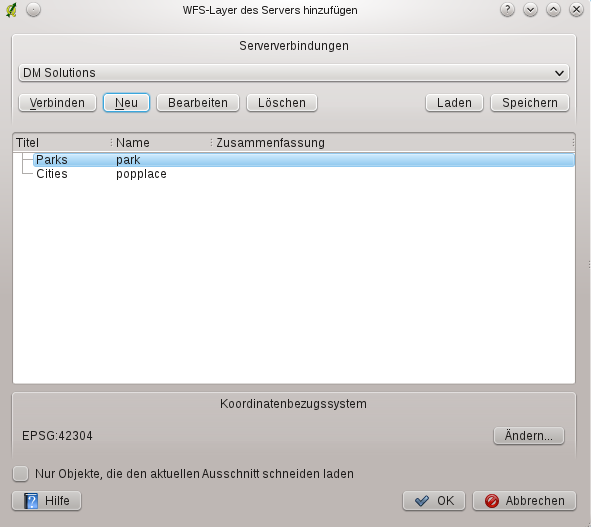
\includegraphics[clip=true,width=0.6\textwidth]{connection_wfs}
  \end{center}
\end{figure}

Si noti che l'avanzamento della ricezione dei dati viene visualizzato nella
parte inferiore sinistra della finestra principale di QGIS. 
Quando il layer è caricato, è possibile identificare e selezionare alcuni
elementi e visualizzare la tabella attributi.

Tenere a mente che il plugin funziona al meglio con server WFS basati su UMN
MapServer. Sono ancora possibili comportamenti anomali e blocchi del plugin,
ma ci saranno miglioramenti in future versioni.

\begin{Tip}[ht]\caption{\textsc{Trovare server WMS e WFS}}
\qgistip{È possibile trovare ulteriori server WMS e WFS usando Google o altro
motore di ricerca preferito. Ci sono anche diversi elenchi di URL pubblici,
alcuni dei quali aggiornati e altri non più mantenuti.
\index{WFS!server remoto!}
}
\end{Tip} 

